\documentclass[10pt,a4paper]{article}
\usepackage[utf8]{inputenc}
\usepackage[italian]{babel}
\usepackage{amsmath}
\usepackage{amsfonts}
\usepackage{amssymb}
\usepackage{graphicx}
\usepackage[left=2cm,right=2cm,top=2cm,bottom=2cm]{geometry}
\newcommand{\rem}[1]{[\emph{#1}]}
\newcommand{\exn}{\phantom{xxx}}

\author{Gruppo 1.BN \\ Massimo Bilancioni, Alessandro Foligno, Giuseppe Zanichelli }
\title{Es02B:Circuito RC - Filtri passivi}
\begin{document}
\date{17 ottobre 2018}
\maketitle


\section{Filtro Passa-basso}
\subsection{}

I valori misurati sono: $R_1  = (3.24\pm 0.03 )K\Omega$ e  $C_1  = (9.7\pm 0.4 )nF$.

a) La frequenza di taglio teorica è  $f_T = 1/2\pi R_1 C_1$ che in base ai valori viene $f_T = (5.1\pm 0.2)KHz$\\
\vspace{0.5cm}

b) A bassa frequenza la funzione di guadagno vale \[A\simeq 1-\frac{f^2}{2f_t^2}\] dove la condizione è \[2\pi RCf\ll1\]
c)Per $f= 2kHz$ il guadagno  vale \[A_{V(teo)}=0.93\pm0.01\]
d)Per $f=20kHz$ il guadagno vale \[A_{V(teo)}=0.24\pm0.01\]. 

Notiamo che nei punti c) e d) non siamo nel regime di basse frequenze e non possiamo usare la formula del punto b).
\subsection{}

a)

b)

 Partitore con resistenze da circa 1~k
Valori misurati $R_1$ e $R_2$ e valore atteso di $A_\mathrm{exp}$:
\[
R_1 = (0.988  \pm0.008  ) \,\mathrm{k}\Omega, \quad
R_2 = (1.187 \pm 0.01 ) \,\mathrm{k}\Omega, \quad
A_\mathrm{exp} = ( 0.544 \pm 0.002 ) 
\]




\subsection{}

\begin{table}[h]
	\centering
	\begin{tabular}{|c|c|c|c|c|c|}
		\hline 
		 VOUT/VIN & $\sigma$ VOUT/VIN  &f [kHz] & $\sigma$ f [kHz]\\
		\hline 
	1.0 & 0.03 & 0.1 & 0.001\\
	0.97 & 0.03 & 1.065 & 0.01\\
	0.96 & 0.04 & 1.49 & 0.01\\
	0.92 & 0.03 & 2.085 & 0.02\\
	0.90 & 0.03 & 2.51 & 0.01\\
	0.87 & 0.03 & 3.01 & 0.01\\
	0.81 & 0.02 & 3.51 & 0.01\\
	0.78 & 0.02 & 3.968 & 0.01\\
	0.75 & 0.02 & 4.428 & 0.01\\
	0.71 & 0.02 & 5.005 & 0.01\\
	0.67 & 0.02 & 5.601 & 0.01\\
	0.65 & 0.02 & 6.038 & 0.01\\
	0.59 & 0.02 & 7.09 & 0.01\\
	0.960 & 0.008 & 0.939 & 0.028\\
	0.790 & 0.002 & 3.71 & 0.11\\
	0.497 & 0.003 & 8.97 & 0.27\\
	0.255 & 0.003 & 19.2 & 0.6\\
	0.0790 & 0.0003 & 66.0 & 2\\
	0.0406 & 0.0003 & 135.0 & 4\\
	0.0184 & 0.0003 & 299.0 & 9\\
	0.0103 & 0.0006 & 53.2*10 & 1.6*10\\
	0.0065 & 0.0002 & 90.5*10 & 3.0 *10\\
		\hline 
	\end{tabular} 
	\caption{(2.b) Tabella con i dati presi e i relativi errori (sono i dati usati per costruire il grafico). Dato che $V_{in}$ lo si è tenuto costante il suo errore sistematico è l'errore di scala della lettura, che nel diagramma di Bode ha l'effetto di traslare tutte le misure nel grafico di una quantità $\sigma_A=\frac{20 \sigma_{V_{in}}}{V_{in} ln(10)} [dB]=0.26 dB$ \label{t:par1}}
\end{table}

\begin{figure}[h]
	\centering
	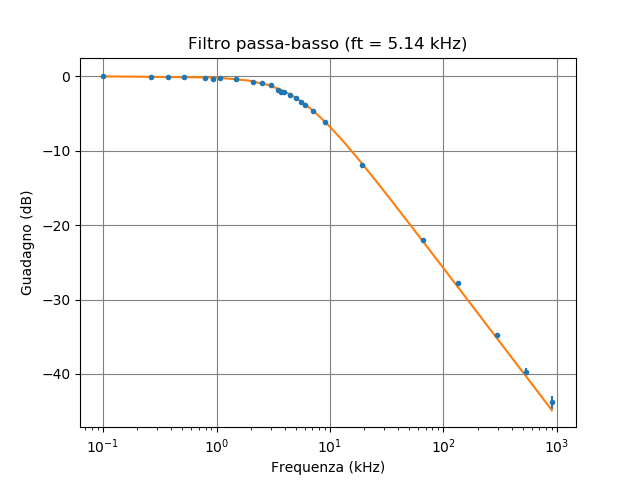
\includegraphics[scale=0.5]{Figure_0.png}

	
	\caption{(2.b) Diagramma di Bode, la linea arancione rappresenta l'andamento atteso con i valori di R e C misurati \label{f:par1}}
\end{figure}
a) l'attenuazione misurata vale, a $2kHz$:
\[A=0.92\pm0.03\]
a $20kHz$:
\[A=0.245\pm0.003\]
b)
    i) Il valore misurato di $f_T$ nel primo modo è: \[f_{T,A}=5.50kHz\pm0.1\]
     Il valore di $f_T$ riportato nel titolo è, invece, stato ottenuto tramite fit del modello esatto effettuato con il modulo curvefit.optimize di scipy.

	ii) $+$ c) 
\begin{figure}[h]
	\centering
	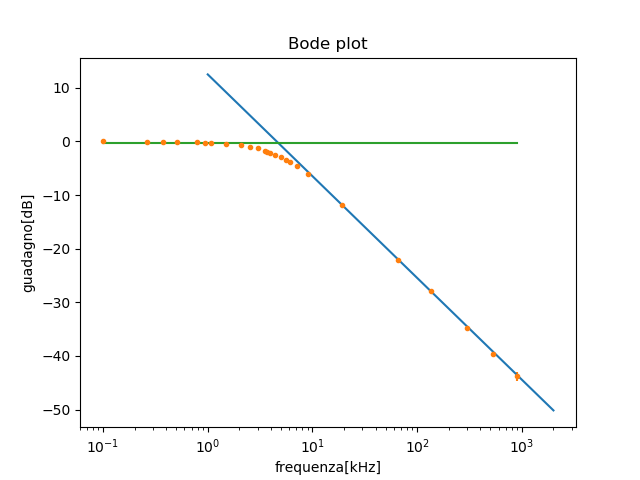
\includegraphics[scale=0.6]{Figure_2.png}
\end{figure}
Per propagare l'errore sull'intersezione scriviamo $f_t(a,b,c)=(c-b)/a$, dove $a,b,c$ sono i parametri di fit delle due rette; la prima retta è $y=c$, la seconda $y=ax+b$. Dopodichè faccio la varianza di quest'espressione considerando errori piccoli e la correlazione fra $a$ e $b$.
La formula ricavata per la varianza di $\log_{10}(f_T)$ è:\[\frac{\sigma_{b}^2}{a^2}+\frac{\sigma^2_a(c-b)^2}{a^4}+\frac{\sigma^2_c}{a^2}+2\frac{\sigma_{ab}^2(b-c)}{a^3}\]
Svolgendo i conti, viene $f_{T,B}=4.7\pm0.6$.

L'incertezza così elevata discende principalmente dal termine che tiene conto della  correlazione fra $a$ e $b$. Per ridurne il valore avremmo dovuto prendere molti più punti ad alte frequenze.

\clearpage


\subsection{}

La misura del tempo di salita è $ t_{sal} = (70\pm 5)\mu s$
\[ f_t = \frac{1.1}{\pi t_{sal}} = (5.00 \pm 0.36) kHz \]

\subsection{}
a) l'impedenza di ingresso del circuito è
\begin{itemize}

\item a bassa frequenza  infinita, è un circuito aperto per la presenza del condensatore.
\item ad alta frequenza $Z_{circuito}\sim R_1$, perchè l'impedenza del condensatore è trascurabile
\item alla frequenza di taglio  $Z_{circuito} = R_1(1-j)$.

\end{itemize}


\vspace{0.5cm}

b)  Se $R_c$ è la resistenza di carico e $A_1$ la funzione di trasferimento del passa-basso senza il carico,  la nuova funzione di trasferimento diventa:
\[ A_{1c} = v_{out}/v_{in}= \frac{A_1}{1+\frac{R_1}{R_c}A_1}\]

Si vede che $A_{1c} \sim A_{1}$ nel limite in cui $R_1 \ll R_c$, che risulta ragionevolmente vero per $R_c = 100 k\Omega$.

Nel caso in cui $R_c = 10 \, k\Omega$, $A_{1c}$ è sensibilmente diversa da $A_1$, in particolare: 

max $|A_{1c}|= \frac{1}{1+R_1/R_C}=0.755$ (il guadagno massimo è minore di 1) e la frequenza di taglio  aumenta $f_{tc}= 1.18 f_{t}$.

\section{Filtro passa-banda}
\subsection{}

a)I valori misurati di  $R_2$ e  $C_2$ sono $R_2  = (3.28 \pm 0.03 )k\Omega$ e  $C_2  = (102\pm 4 )nF$
\vspace{0.5cm}

b) Dalle misure risulta $A_2 = (1,00- 0.01)$ e  $f_2 = ( 491\pm 7) Hz$. 

Ci si aspetta che il massimo guadagno ad alta frequenza sia  uguale a $1$, mentre la frequenza di taglio attesa è: \[ f_{2,Att}  = 1/(2\pi R_2 C_2)= ( 476\pm 19) Hz\]
\subsection{}

a) tramite le misure si è trovato $A_0 =(0.479\pm 0.008)$, $f_L = (234\pm 2) Hz$ e $ f_{H} = (10.6\pm 0.1) kHz$.

I valori attesi sono rispettivamente $A_{0,Att} = \frac{1}{1+R_1/R_2}= 0.503\pm 0.005$ (l'incertezza deriva dall'errore sul rapporto delle resistenze) , $f_{L,Att} = \frac{1}{2}f_2= (238\pm 10) Hz$ e $ f_{H,Att}=2 f_1 = (10.2\pm 0.4) kHz$ (in realtà il rapporto $R_1/R_2$ con il relativo errore modifica l'incertezza sulle frequenze attese che quindi sarà sicuramente più grande).
L'errore su $A_0 $ si è stimato guardando la minima variazione del cursore sull'oscilloscopio, l'errore su $f_L$ e $f_H$ si è ottenuto guardando l'intervallo di frequenze in cui l'ampiezza sull'oscilloscopio restava quella voluta.
\vspace{0.5cm}


b) La funzione di trasferimento totale del circuito è \[A_{tot}= \frac{A_1A_2}{1+\frac{R_1}{R_2}A_1A_2}\]
essendo nel nostro caso $R_1 \simeq R_2$, \[A_{tot}\simeq \frac{A_1A_2}{1+A_1A_2}\] di conseguenza il guadagno massimo è $1/2$.

Se $\omega \ll \omega_1 $ allora $A_1\simeq 1 $ e \[A_{tot}\simeq \frac{A_2}{1+A_2}= \frac{1}{2}\frac{j\omega/(\omega_2/2)}{1+j\omega/(\omega_2/2)}\] da cui si vede che  la frequenza di taglio teorica più bassa del passa-banda  risulta $f_L = \frac{1}{2}f_2$.

Si fa un discorso analogo nel caso  $\omega \gg \omega_2 $ per trovare che la frequenza di taglio teorica più alta è $f_H = 2f_1$

Si ha come ci si aspetta un allargamento della banda.
\vspace{0.5cm}

c) Si ha  $A_{tot}\simeq A_1A_2$ nel limite in cui $R_2 \gg R_1$, in questo limite l'impedenza del carico relativo al passa-basso è così grande che si può approssimare con un circuito aperto e quindi i fue filtri si possono considerare in cascata.







\section*{Dichiarazione}
I firmatari di questa relazione dichiarano che il contenuto della relazione \`e originale, con misure effettuate dai membri del gruppo, e che tutti i firmatari hanno contribuito alla elaborazione della relazione stessa.

\end{document}